\documentclass{llncs}

\usepackage{cite}
\usepackage{xspace}
\usepackage{hyperref}
\usepackage{xcolor}
\usepackage{graphicx}

\newcommand{\jkind}{{\sc JKind}\xspace}
\newcommand{\kind}{{\sc Kind}\xspace}
\newcommand{\pkind}{{\sc PKind}\xspace}
\newcommand{\jkindapi}{{\sc JKindApi}\xspace}
\newcommand{\lustre}{{\sc Lustre}\xspace}
\newcommand{\spear}{{\sc SpeAR}\xspace}
\newcommand{\simpal}{{\sc SIMPAL}\xspace}
\newcommand{\limp}{{\sc Limp}\xspace}
\newcommand{\agree}{{\sc AGREE}\xspace}
\newcommand{\gryphon}{{\sc Gryphon}\xspace}
\newcommand{\nuxmv}{{\sc nuXmv}\xspace}
\newcommand{\zustre}{{\sc Zustre}\xspace}
\newcommand{\yices}{{\sc Yices}\xspace}
\newcommand{\zthree}{{\sc Z3}\xspace}

\newcommand{\todo}[1]{{\color{red} #1}}

\renewcommand{\paragraph}[1]{\vspace{5pt}\noindent {\bf #1}}
\newcommand{\application}[2]{
  \paragraph{#1} \hfill {\it #2}
  \vspace{1pt}
}

\newcommand{\mike}[1]{\textcolor{red}{#1}}

\title{The JKind Model Checker}
\author{ Authors anonymized for submission to CAV 2018
%  Andrew Gacek\inst{1} \and
%  John Backes\inst{1} \and
%  Mike Whalen\inst{2} \and
%  Lucas Wagner\inst{1} \and
%  Elaheh Ghassabani\inst{2}
  }
\institute{ Institute anonymized for submission to CAV 2018
%  Rockwell Collins \\
%  \email{andrew.gacek@gmail.com}, \email{lucas.wagner@rockwellcollins.com}
%  \and
%  Amazon Web Services \\
%  \email{john.backes@gmail.com}
%  \and
%  University of Minnesota
%  \email{ghass013@umn.edu}, \email{mwwhalen@umn.edu}
}

\begin{document}
\maketitle

\begin{abstract}
  \jkind is an open-source industrial model checker 
  %developed by
  %Rockwell Collins and the University of Minnesota. 
  \jkind uses
  multiple parallel engines to prove or falsify safety properties of
  infinite state models. It is portable, easy to install, performance competitive with other state-of-the-art model checkers, and has features designed to improve the results presented to users: {\em inductive validity cores} for proofs and {\em counterexample smoothing} for test-case generation.  It serves as the back-end for
  various industrial applications.
\end{abstract}

\section{Introduction}

\jkind is an
open-source\footnote{Site information for download anonymized for submission to CAV 2018 - tool is available in artifact submission %\url{https://github.com/agacek/jkind}
} industrial
infinite-state inductive model checker for safety properties. Models
and properties in \jkind are specified in
\lustre~\cite{halbwachs1991ieee}, a synchronous data-flow language,
using the theories of linear real and integer arithmetic. \jkind uses
SMT-solvers to prove and falsify multiple properties in parallel.
%
A distinguishing characteristic of \jkind is its focus on the usability  of results. For a proven property, \jkind provides traceability between the property and individual model elements. For a falsified property, \jkind provides options for simplifying the
counterexample in order to highlight the root cause of the failure. In industrial applications, we have found these additional usability aspects to be at least as important as the primary results.
%
Another important characteristic of \jkind is that is it designed to be integrated directly into user-facing applications. Written in Java, \jkind runs on all major platforms and is easily compiled into other Java applications. \jkind bundles the Java-based {\sc SMTInterpol} solver and has no external dependencies. However, it can optionally call \zthree, \yices 1, \yices 2, {\sc CVC4}, and {\sc
  MathSAT} if they are available.

\section{Functionality and Main Features}

\begin{figure}
  \begin{center}
    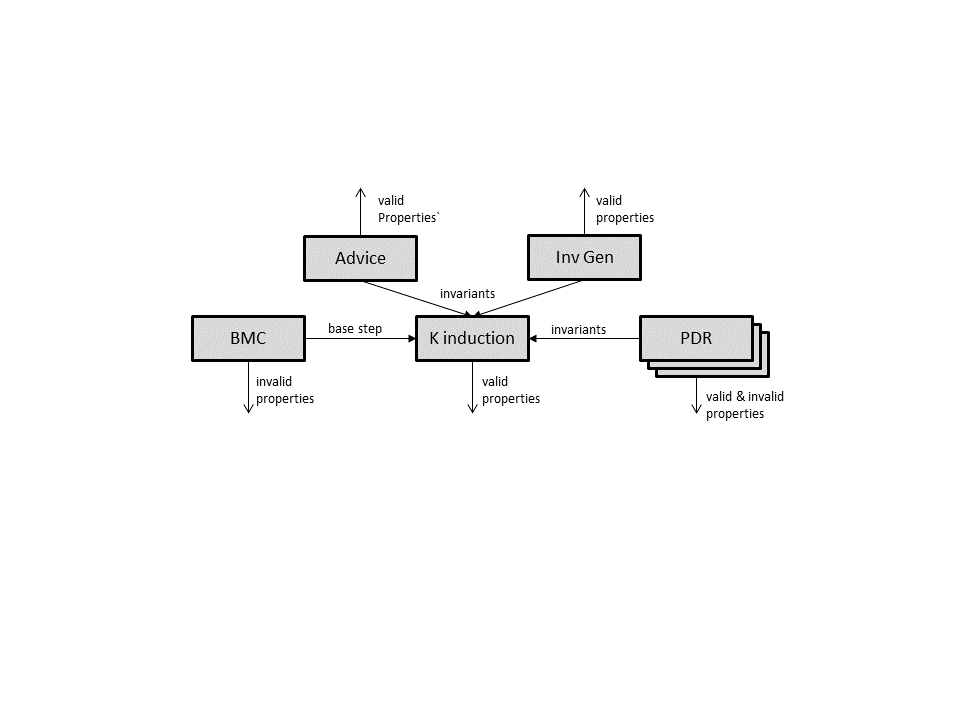
\includegraphics[clip,trim=140 220 100 140,scale=0.6]{engines.png}
  \end{center}
  \vspace{-2em}
  \caption{\jkind engine architecture}
  \vspace{-1em}
 % \mike{Shrink figure vertically}
  \label{fig:engines}
\end{figure}

\jkind is structured as several parallel engines that coordinate to
prove properties, mimicking the design of \pkind and \kind 2~\cite{champion2016cav, kahsai2011pdmc}.
Some engines are directly responsible for proving properties, others aid that effort by generating invariants, and still others are reserved for post-processing of proof or counterexample results. Each engine can be enabled or disabled separately based on the user's needs. The architecture of \jkind allows any engine to broadcast information to the other engines (for example, lemmas, proofs, counterexamples) allowing straightforward integration of new functionality.

The solving engines in \jkind are:  (1) \textbf{Bounded Model Checking (BMC).} The BMC engine performs a standard iterative unrolling of the transition relation to find counterexamples and to serve as the base case of $k$-induction. The BMC engine guarantees that any counterexample it finds is minimal in length. (2) \textbf{$k$-induction.} The $k$-induction engine performs the inductive step of $k$-induction, possibly using invariants generated by other engines. \textbf{Invariant Generation.} The invariant generation engine uses a template-based invariant generation technique~\cite{kahsai2012nfm} using its own $k$-induction loop. (3) \textbf{Property Directed Reachability (PDR).} The PDR engine performs property directed reachability~\cite{een2011fmcad} using the implicit abstraction technique~\cite{cimatti2014tacas}. Unlike BMC and $k$-induction, each property is handled separately by a different PDR sub-engine. %Invariants generated as a side-product of PDR are shared with the $k$-induction process.

Invariant sharing between the solvers (shown in Figure~\ref{fig:engines}) is an important part of the architecture.  In our internal benchmarking, we have found that implicit abstraction PDR performs best when operating over a single property at a time and without use of lemmas generated by other approaches.  On the other hand, the invariants generated by PDR and template lemma generation often allow $k$-induction, which operates on all properties in parallel, to substantially reduce the verification time required for models with large numbers of properties.  %As described in Section~\ref{sec:benchmarks}, \jkind\ is competitive with other tools

\subsection{Post Processing and Re-verification}

A significant part of the research and development effort for \jkind\ has focused on
post-processing results for presentation and repeated verification of models under development.

%and supporting re-verification of slightly-modified models.  Simplifying counterexamples to support root-cause analysis and providing traceability information to automatically create traceability matrices and determine adequacy of requirements has been important in the industrial use of the tools.  Additionally, this type of coverage and traceability information is often required for certification of safety critical systems~\cite{DO178C}.  To support these uses,

\paragraph{Inductive Validity Cores (IVC).} For a proven property, an inductive validity core is a subset of \lustre equations from the input model for which the property still
holds~\cite{ghassabani2016fse,Ghass17AllIVCs}.  Inductive validity cores can be used for traceability from property to model elements and determining coverage of the model by a set of properties~\cite{Ghass17Cov}.  This facility can be used to automatically generate traceability and adequacy information (such as traceability matrices~\cite{fifarek2017nfm} important to the certification of safety-critical avionics systems~\cite{DO178C}).
The IVC engine uses a heuristic algorithm to efficiently produce minimal or nearly minimal cores.   In a recent experiment over a superset of the benchmark models described in the experiment in Section~\ref{sec:experiment}, we found that our heuristic IVC computation added 31\% overhead to model checking time, and yielded cores approximately 8\% larger than the guaranteed minimal core computed by a very expensive ``brute force'' algorithm.  As a side-effect, the IVC algorithm also minimizes the set of invariants used to prove a property and emits this reduced set to other engines (notably the {\em Advice} engine, described below).

%Since \lustre is 

\paragraph{Smoothing.}  To aid in counterexample understanding and in
creating structural coverage tests that can be more easily explained,
\jkind provides an optional post-processing step to minimize the
number of changes to input variables---{\em smoothing} the
counterexample.  For example, applied to 129 test cases generated for
a production avoinics flight control state machine, smoothing
increased runtime by 40\% and removed 4 unnecessary input changes per
test case on average.  The smoothing engine uses a {\sc MaxSat} query
over the original BMC-style unrolling of the transition relation
combined with weighted assertions that each input variable does not
change on each step. The {\sc MaxSat} query tries to satisfy all of
these weighted assertions, but will break them if needed. This has the
effect of trying to hold all inputs constant while still falsifying
the original property and only allowing inputs to change when
needed. This engine is only available with SMT-solvers that support
{\sc MaxSat} such as \yices 1 and \zthree.

\paragraph{Advice.} The advice engine saves and re-uses the invariants that were used by \jkind to prove the properties of a model.  Prior to analysis, \jkind\ performs model slicing and flattening to generate a flat transition-relation model.  Internally, invariants are stored as a set of proven formulas (in the \lustre syntax) over the variables in the flattened model.  An {\em advice} file is simply the emitted set of these invariant formulas.  When a model is loaded, the formulas are loaded into memory. Formulas that are no longer syntactically or type correct are discarded, and the remaining set of formulas are submitted as an initial set of possible invariants to be proved via $k$-induction. If they are proved, they are passed along to other engines; if falsified, they are discarded.
%
Names constructed between multiple runs of \jkind are stable, so if a
model is unchanged, it can be usually be re-proved quickly using the
invariants and $k$-induction.  If the model is slightly changed, it is
often the case that most of the invariants can be re-proved, leading
to reduced verification times.

If the IVC engine is also enabled, then advice emits a (close to) minimal set of lemmas used for proof; this often leads to faster re-verification (but more expensive initial verification), and can be useful for examining which of the generated lemmas are useful for proofs.

\section{Experimental Evaluation}
\label{sec:experiment}
We evaluated the performance of \jkind against \kind
2~\cite{champion2016cav}, \zustre~\cite{Zustre}, Generalized PDR in
\zthree~\cite{GPDR}, and IC3 in \nuxmv~\cite{cimatti2014tacas}, Our
benchmark suite comes from~\cite{cimatti2014tacas} and contains 688
models over the theory of linear integer arithmetic\footnote{Available
  at:
  \url{https://es.fbk.eu/people/griggio/papers/tacas14-ic3ia.tar.bz2}.
  Note that we removed 263 duplicate benchmarks from the original
  set.}.  All the experiments have been performed on a 64-bit Ubuntu
17.10 Linux machine with a 12-core Intel Xeon CPU E5-1650 v3 @
3.50GHz, with 32Gb of RAM and a time limit of 60 seconds per model.

Performance for \jkind and related solvers is shown in
Figure~\ref{fig:benchmark}. The key describes the number of benchmarks
solved for each tool, and the graph shows the aggregate time required
for solving, ordered by time required per-problem, ordered
independently for each tool. \jkind was able to verify or falsify the
most properties, although \zthree was often the fastest tool.  We note
that many of the benchmarks in this set are quickly evaluated: \zthree
solves the first 400 benchmarks in 10 seconds.  Due to \jkind's use of
Java and multiple threads, the JVM/\jkind startup time for an empty
model is approximately 0.35s, which leads to poor performance on small
models\footnote{Without startup time, the curve for \jkind is close to
  the curve for \zustre}.  As always, benchmarks should be taken with
a large grain of salt.  In~\cite{champion2016cav}, a different set of
benchmarks favored \kind2.  We believe that all the solvers are
relatively competitive.


\begin{figure}
  \begin{center}
    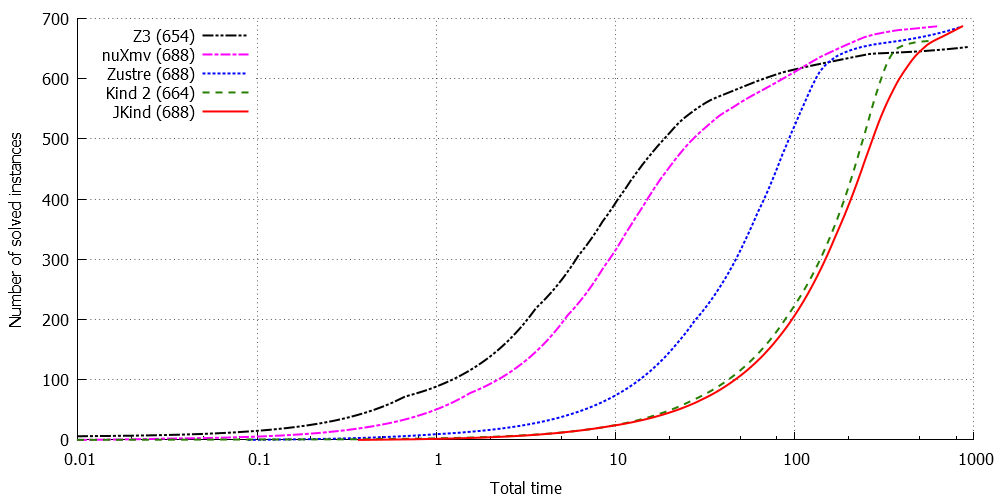
\includegraphics[width=\textwidth]{graph.png}
  \end{center}
  \vspace{-2em}
  \caption{Performance benchmarks}
  \vspace{-1em}
  \label{fig:benchmark}
\end{figure}


\section{Integration \& Applications}

%\mike{Should we talk less (and less repetitively) about each table and use a chart that describes the jkind features used for each tool?}

\jkind is the back-end for a variety of user-facing applications. In this section, we briefly highlight a few of these applications and how they employ the features discussed previously.
%
%We wrote \jkind in Java which makes it multi-platform and very easy to
%integrate into other Java applications. Moreover, we created the
%\jkindapi package which contains utilities for creating \lustre
%specifications, calling \jkind, processing \jkind results, graphically
%displaying real-time results, and nicely formatting counterexamples.
%Many of the applications in this section make heavy use of \jkindapi.
%

(1) The {\em Specification and Analysis of Requirements} (\spear) tool is an open source tool for prototyping and analysis of requirements~\cite{fifarek2017nfm}.  Starting from a set of formalized requirements, \spear uses \jkind to determine whether or not the requirements meet certain {\em properties}.  It uses IVCs to create a traceability matrix between requirements and properties, highlighting unused requirements, over-constrained properties, and other common problems. \spear also uses \jkind with smoothing for test case generation using the Unique First Cause criteria~\cite{whalen2006issta}.
%
%\spear captures
%requirements in a way that is backed by the formal semantics of
%\lustre, which enables them to be analyzed using model checking to
%ensure they are correct and consistent.
%
%\spear uses \jkind to prove properties over requirements, and uses IVC
%to create a traceability matrix between requirements and properties.
%This quickly highlights unused requirements, over-constrained
%properties, and other common problems. \spear also uses \jkind for
%test case generation using the Unique First Cause
%criteria~\cite{whalen2006issta} by creating {\em trap properties}.
%Each trap property is expected to be falsifiable, but in such a way
%that the counterexample has exactly the desired properties for a given
%test case. \spear uses smoothing in \jkind to ensure the resulting
%test cases are simple and understandable.

(2) The {\em Assume Guarantee Reasoning Environment} (\agree)~\cite{cofer2012nfm,QFCS15:backes,hilt2013} is an open-source compositional verification tool that proves properties of hierarchically-composed models in the Architectural Analysis and Design Language (AADL) language.  %\jkind as the default model checker for AGREE.
%
%\application{Assume Guarantee Reasoning Environment}{Open Source}
%
%\noindent \jkind is used as the default model checker for the Assume
%Guarantee Reasoning Environment (\agree)~\cite{cofer2012nfm}. \agree
%refers to both an embedded language annex in the Architectural
%Analysis and Design Language (AADL) and to a plugin for the OSATE AADL
%Integrated Development Environment. The \agree annex annotates the
%AADL model with formal requirements, and the plugin reasons about
%these requirements. The purpose of \agree is to model behavioral
%requirements of an embedded system using formal assume guarantee
%contracts. The plugin generates Lustre specifications that are checked
%by \jkind.
%
\agree makes use of multiple \jkind features including smoothing to
present clear counterexamples, IVC to show requirements traceability,
and counterexample generation to check the consistency of an AADL
component's contract. \agree also uses \jkind for test-case generation
from component contracts.

%\application{Static IMPerative AnaLyzer}{Open Source}
(3) The {\em Static IMPerative AnaLyzer} (\simpal) is a tool for
performing compositional reasoning over
software~\cite{wagner2017spin}. \simpal is based on \limp, a \lustre-like imperative language with extensions for control flow elements, global variables, and a syntax for specifying preconditions, postconditions, and global variable interactions of
preexisting components. \simpal translates \limp programs to an
equivalent \lustre representation which is passed to \jkind to
perform assume-guarantee reasoning, reachability, and viability
analyses. 
%The feedback from these analyses is used to refine the
%program to ensure that the software functions as intended.

\jkind is also used by two proprietary tools used by product areas within a company\footnote{Organization anonymized for submission}.  The first is a {\em Mode Transition Table} verification tool used for the complex state machines which manage flight modes of an aircraft.
\jkind is used to check properties and generate tests for mode and transition coverage from \lustre models generated from the state machines.
IVCs are used to establish traceability, i.e. which transitions are covered by which properties.  The second is a {\em Crew Alerting System} MC/DC test-case generation tool for a proprietary DSL used for messages and alerts to airplane pilots.  Smoothing is very important in this context as test cases need to be run on the actual hardware where
timing is not precisely controllable. Thus, test cases with a minimum
of changes to the inputs are ideal.
%
%These state
%machines often have few states, but hundreds of possible transitions between
%states. There is a priority ordering to resolve conflicts between
%transitions, but this can make it hard to fully exercise the behavior
%of a state machine. The flight controls group has developed a
%particular graphical representation to manage this complexity.
%
%We have developed a tool which formalizes these state machine models.
%Trap properties are used to generate test cases exercising all transitions. Here IVCs are used when a trap property is {\em valid}, which means it failed to generate a test case. The IVC indicates which
%transitions are blocking the transition we wish to exercise in the
%test case. The tool presents all this information graphically to its
%users.

% \application{MC/DC Test Case Generation}{Proprietary}

% \noindent An engineering group at Rockwell Collins develops equations
% which determine which messages and alerts should be delivered to
% pilots. Certification for this system requires extensive test cases
% which must satisfy criteria such as the Modified Condition/Decision
% Coverage (MC/DC) metric. We have developed a tool which generates
% these tests by translating the equations into \lustre and generating
% MC/DC trap properties in \jkind. Smoothing is very important in this
% context as test cases need to be run on the actual hardware where
% timing is not precisely controllable. Thus, test cases with a minimum
% of changes to the inputs are ideal.

% \application{Model-based Fuzzing}{Open Source}

% \noindent As part of an ongoing DARPA program, Rockwell Collins is
% developing a tool for generating fuzz tests from system models. This
% tool takes a \lustre description of a system and uses \jkind to
% generate test cases which exercise different portions of the model.
% Effective fuzz testing requires a huge number of test cases which is
% not feasible to generate solely with a model checker. Instead, this
% fuzzing tool uses interval generalization in \jkind to generate
% generalized counterexamples which it then randomly samples at high
% speed. In fact, research in this area has recently expanded interval
% generalization to trapezoidal generalization which is strictly more
% general, but still allows very fast random sampling.

% \paragraph{The \gryphon Framework.} The Rockwell Collins \gryphon
% framework~\cite{miller2010cacm} translates Simulink models to various
% analysis tools for verification and testing. \gryphon uses the \lustre
% language internally which was the originally motivation for \kind
% (and eventually \jkind) to accept \lustre. As \gryphon is the only
% application in our list which does not directly integrate \jkind, it
% does not specifically use any features of \jkind. Still, features like
% smoothing and IVC have been successfully used in combination with
% \gryphon to great effect.

\section{Related Work}
\jkind is one of a number of similar infinite-state inductive model
checkers including {\sc Kind 2}~\cite{champion2016cav},
\nuxmv~\cite{cimatti2014tacas}, \zthree with generalized
PDR~\cite{GPDR}, and \zustre~\cite{Zustre}. They operate over a
transition relation described either as a \lustre program (\kind 2,
\jkind, and \zustre), an extension of the SMV language (\nuxmv), or as
a set of Horn clauses (\zthree).  Each tool uses a portfolio-based
solver approach, with \nuxmv, \jkind, and \kind 2 all
supporting both $k$-induction and a variant of PDR/IC3.  \nuxmv also
supports guided reachability and $k$-liveness.  Other tools such as
{\sc ESBMC-DepthK} \cite{rocha2017model}, {\sc VVT}
\cite{beyer2016smt} {\sc CPAchecker}, \cite{beyer2015boosting}, {\sc
  CPROVER} \cite{brain2015safety} use similar techniques for
reasoning about C programs.

We believe that the \jkind IVC support is similar to~\emph{proof-core} support provided by commercial hardware model checkers: Cadence Jasper Gold and Synopsys VC Formal~\cite{hanna2015formal, jasper_gold, Synopsys_VC_formal}.  The proof-core provided by these tools is used for internal coverage analysis measurements performed by the tools.  Unfortunately, the algorithms used in the commercial tool support are undocumented and performance comparisons are prohibited by the tool licenses, so it is not possible to compare performance on this aspect.

There are several tools that support reuse or exchange of verification results, similar to our {\em advice} feature.  Recently, there has been progress on standardized formats~\cite{Beyer:2016} of exchange between analysis tools.  Our current advice format is optimized for use and performance with our particular tool and designed for re-verification rather than exchange of partial verification information.  However, supporting a standardized format for exchanging verification information would be a useful feature for future use.


% \paragraph{Simulation.} To help users and developers to understand
% \lustre specifications, \jkind can compile a \lustre specification
% into an Excel-based simulation. The simulation uses the formula and
% reference language of Excel to compute, in real-time, the output of the
% specification as inputs are entered and manipulated. This spreadsheet
% interface to the specification is satisfyingly capable and versatile.

\section{Conclusion}
\jkind is similar to a number of other solvers that each solve
infinite state sequential analysis problems. Nevertheless, it has some
important features that distinguish it. First, a focus on quality of
feedback to users for both valid properties (using IVCs) and invalid
properties (using smoothing). Second, it is supported across all major platforms and is
straightforward to port due to its implementation in Java. Third, it
is small, modular, and well-architected, allowing straightforward
extension with new engines. Fourth, it is open source with a liberal
distribution license (BSD), so it can be adapted for various purposes,
as demonstrated by the number of tools that have incorporated it.



\paragraph{Acknowledgments}

Acknowledgements anonymized for submission to CAV 2018.

%\noindent The work presented here was sponsored by DARPA as part of the HACMS
%program under contract FA8750-12-9-0179.

\bibliography{main}{}
\bibliographystyle{splncs03}

\end{document}




% Local Variables:
% TeX-master: "main.tex"
% End:

%  LocalWords:  BMC PDR IVC MaxSat Yices SpeAR SIMPAL Gryphon UI JVM
%  LocalWords:  JKindApi natively Kind IMPerative AnaLyzer IVCs IC
%  LocalWords:  postconditions DARPA HACMS NuXmv Zustre
%  LocalWords:  architected
